

\documentclass[12]{fphw}
\usepackage{float}
% Template-specific packages

\usepackage{graphicx} % Required for including images



\usepackage{fullpage,enumitem,amsmath,amssymb,graphicx}
\usepackage{pdfpages}
\usepackage{amsmath} 
% for table
\newcommand\Tstrut{\rule{0pt}{2.6ex}}       % "top" strut
\newcommand\Bstrut{\rule[-0.9ex]{0pt}{0pt}} % "bottom" strut
\newcommand{\TBstrut}{\Tstrut\Bstrut} % top&bottom struts
%----------------------------------------------------------------------------------------
%	ASSIGNMENT INFORMATION
%----------------------------------------------------------------------------------------

\title{Homework \#1} % Assignment title

\author{Ali BaniAsad} % Student name

\date{March 28th, 2025} % Due date

\institute{Sharif University of Technology \\ Institute of Aerospace} % Institute or school name

\class{Optimal Control I} % Course or class name

\professor{Dr. Assadian} % Professor or teacher in charge of the assignment

%----------------------------------------------------------------------------------------

\begin{document}

\maketitle % Output the assignment title, created automatically using the information in the custom commands above
\section*{Problem 1}
\begin{enumerate}[label=(\alph*)]
	\item 
	$z = f(x, y) = y\sin(x+y)-x\sin(x-y)$ \\
Gradient of f(x, y):
$$\vec{\nabla} f = \begin{bmatrix}
	\dfrac{\partial f}{\partial x} \\[6pt]
	\dfrac{\partial f}{\partial y}
\end{bmatrix} $$
$$\vec{\nabla} f = \begin{bmatrix}
	y \cos(x + y) - \sin(x - y) - x  \cos(x - y) \\
	y  \cos(x + y) + \sin(x + y) + x  \cos(x - y)
\end{bmatrix} $$

Two nonlinear equations with two unknowns. We use MATLAB to solve this equations. MATLAB file is attached.
\begin{table}[h]
				\caption {Answers} \label{ans} 
	\begin{center}
		\begin{tabular}{| l | l |}
			\hline
			x & y\\ \hline
			-3.41877 & -1.82764 \\ \hline
			-2.88904 & 1.84693 \\ \hline
			-2.02875 & 0.00000 \\ \hline
			-1.84693 & -2.88904 \\ \hline
			-1.82764 & 3.41877 \\ \hline
			-1.75560 & 0.36547 \\  \hline
			-0.36547 & -1.7556 \\ \hline
			0.00000 & -2.02875 \\ \hline
			0.00000 & 0.00000 \\ \hline
			0.00000 & 2.02875 \\ \hline
			0.36547 & 1.7556 \\ \hline
			1.75560 & -0.36547 \\ \hline
			1.82764 & -3.41877 \\ \hline
			1.84693 & 2.88904 \\ \hline
			2.02875 & 0.00000 \\ \hline
			2.88904 & -1.84693 \\ \hline
			3.41877 & 1.82764 \\ \hline
		\end{tabular}
	\end{center}
\end{table}
Answers are provided in table \ref{ans}


Hessian matrix:
$$H = \dfrac{\partial^2 f}{\partial \vec{X}^2} = \begin{bmatrix}
	\dfrac{\partial^2 f}{\partial x^2} & \dfrac{\partial^2 f}{\partial xy} \\[6pt]
	\dfrac{\partial^2 f}{\partial yx}  & \dfrac{\partial f}{\partial y^2}
\end{bmatrix} $$
$$\vec{\nabla} f = \begin{matrix}
	-y  \sin(x + y) - 2  \cos(x - y) + x  \cos(x -y) & \cos(x + y) - y  \sin(x + y) + cos(x - y) - x  \sin(x - y) \\
	\\cos(x + y) - y \sin(x + y) + \cos(x - y) - x  \sin(x - y)  & x  \sin(x - y) + 2  \cos(x + y) - y  \sin(x + y)
\end{matrix} $$
Hessian matrix and eigenvalues have calculated in MATLAB and attached.
Maximum
Minimum
Saddle Point
\begin{table}[h]
	\caption {Answers With Conditions} \label{ansWithHessian} 
	\begin{center}
		\begin{tabular}{| l | l | l |}
			\hline
			x & y & Point Condition\\ \hline
			-3.41877 & -1.82764 & Maximum \\ \hline
			-2.88904 & 1.84693 & Saddle Point \\ \hline
			-2.02875 & 0.00000 & Saddle Point\\ \hline
			-1.84693 & -2.88904 & Saddle Point\\ \hline
			-1.82764 & 3.41877 & Minimum \\ \hline
			-1.75560 & 0.36547 & Maximum \\  \hline
			-0.36547 & -1.7556 & Minimum \\ \hline
			0.00000 & -2.02875 & Saddle Point\\ \hline
			0.00000 & 0.00000  & Saddle Point\\ \hline
			0.00000 & 2.02875  & Saddle Point\\ \hline
			0.36547 & 1.7556   & Minimum\\ \hline
			1.75560 & -0.36547 & Saddle Point\\ \hline
			1.82764 & -3.41877 & Minimum \\ \hline
			1.84693 & 2.88904 & Saddle Point\\ \hline
			2.02875 & 0.00000 & Saddle Point\\ \hline
			2.88904 & -1.84693 & Saddle Point \\ \hline
			3.41877 & 1.82764 & Maximum\\ \hline
		\end{tabular}
	\end{center}
\end{table}


Answers and conditions are provided in table \ref{ansWithHessian}
\begin{figure}[H]
	\caption{3D figure of function}
	\centering
	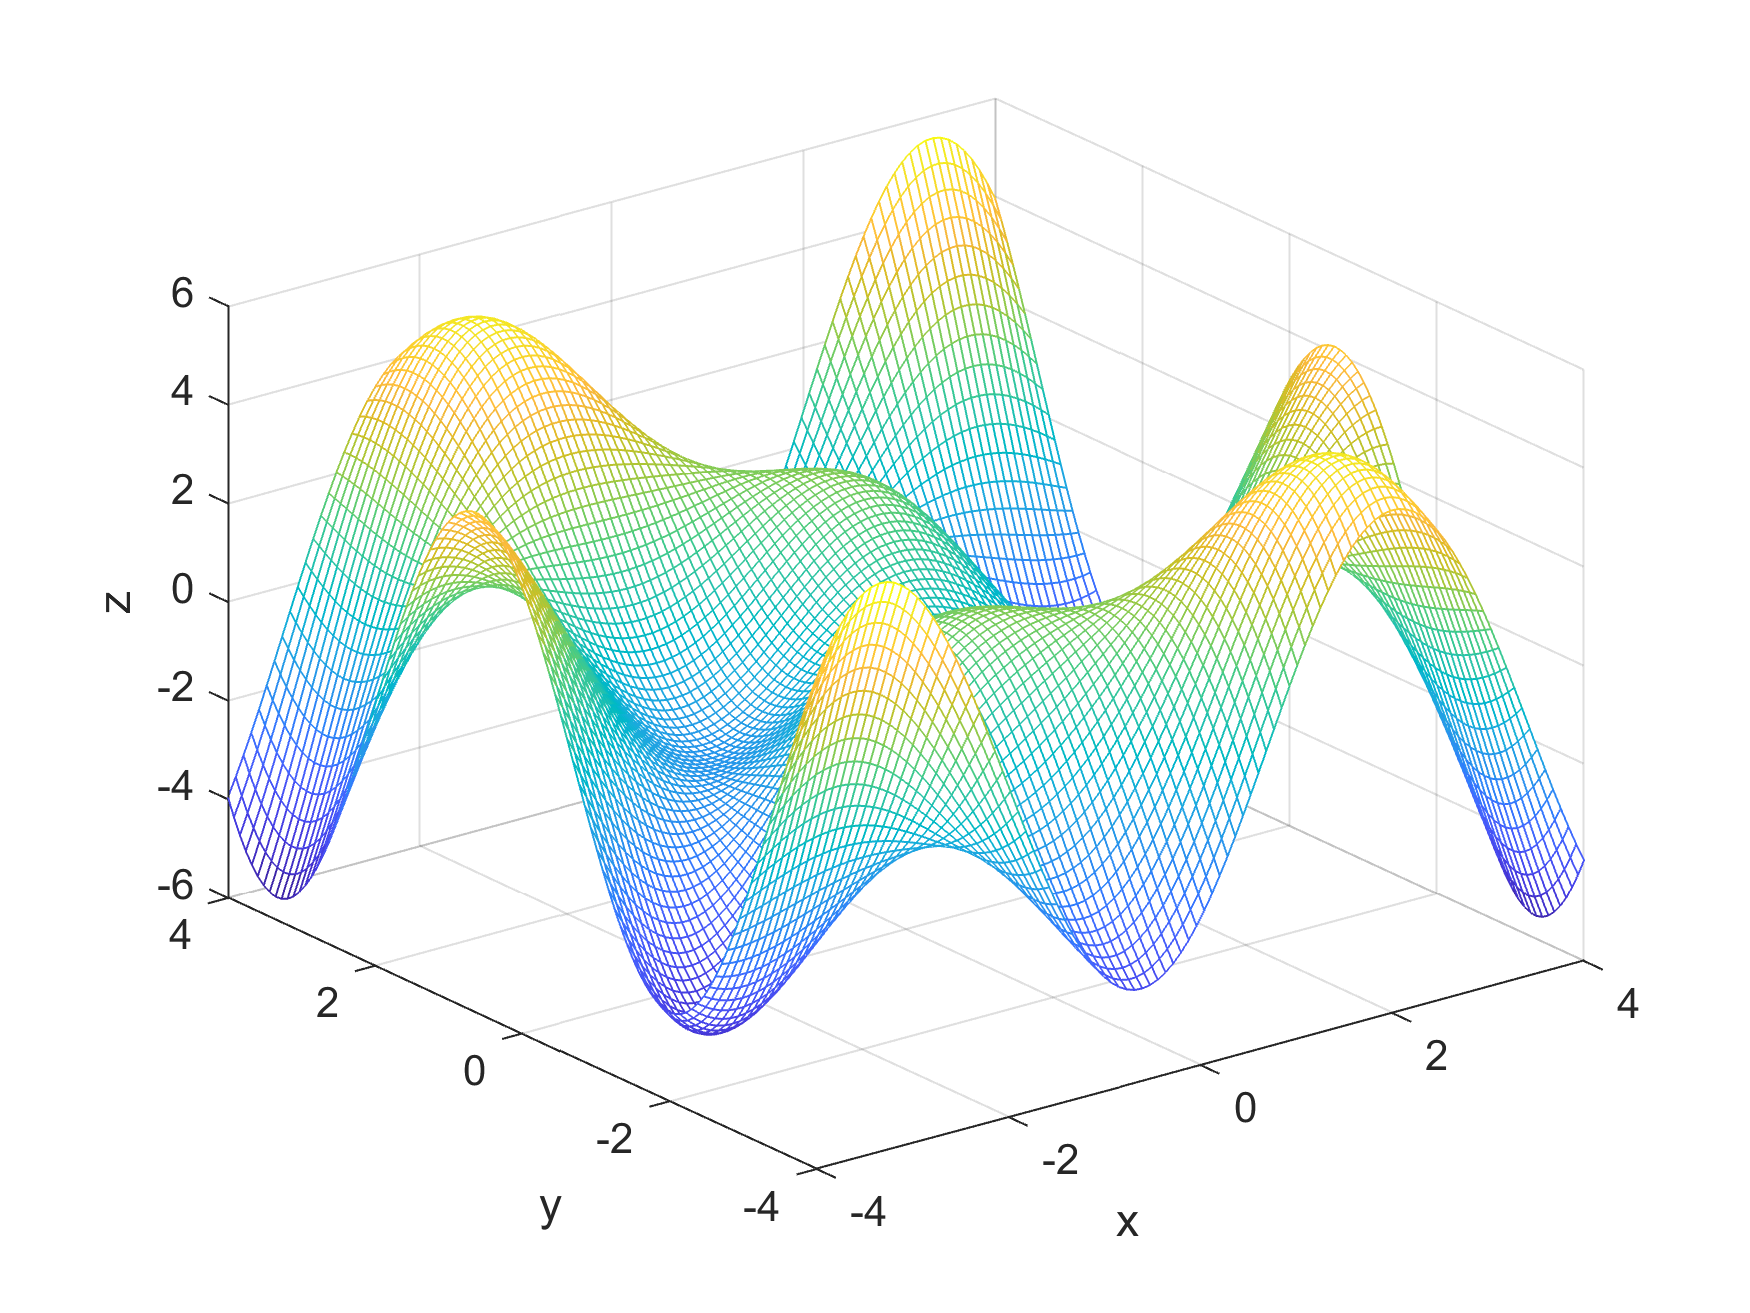
\includegraphics[width=12cm]{Q1/figures/3Dplot.png}
\end{figure}
\begin{figure}[H]
	\caption{3D figure of function with Points}
	\centering
	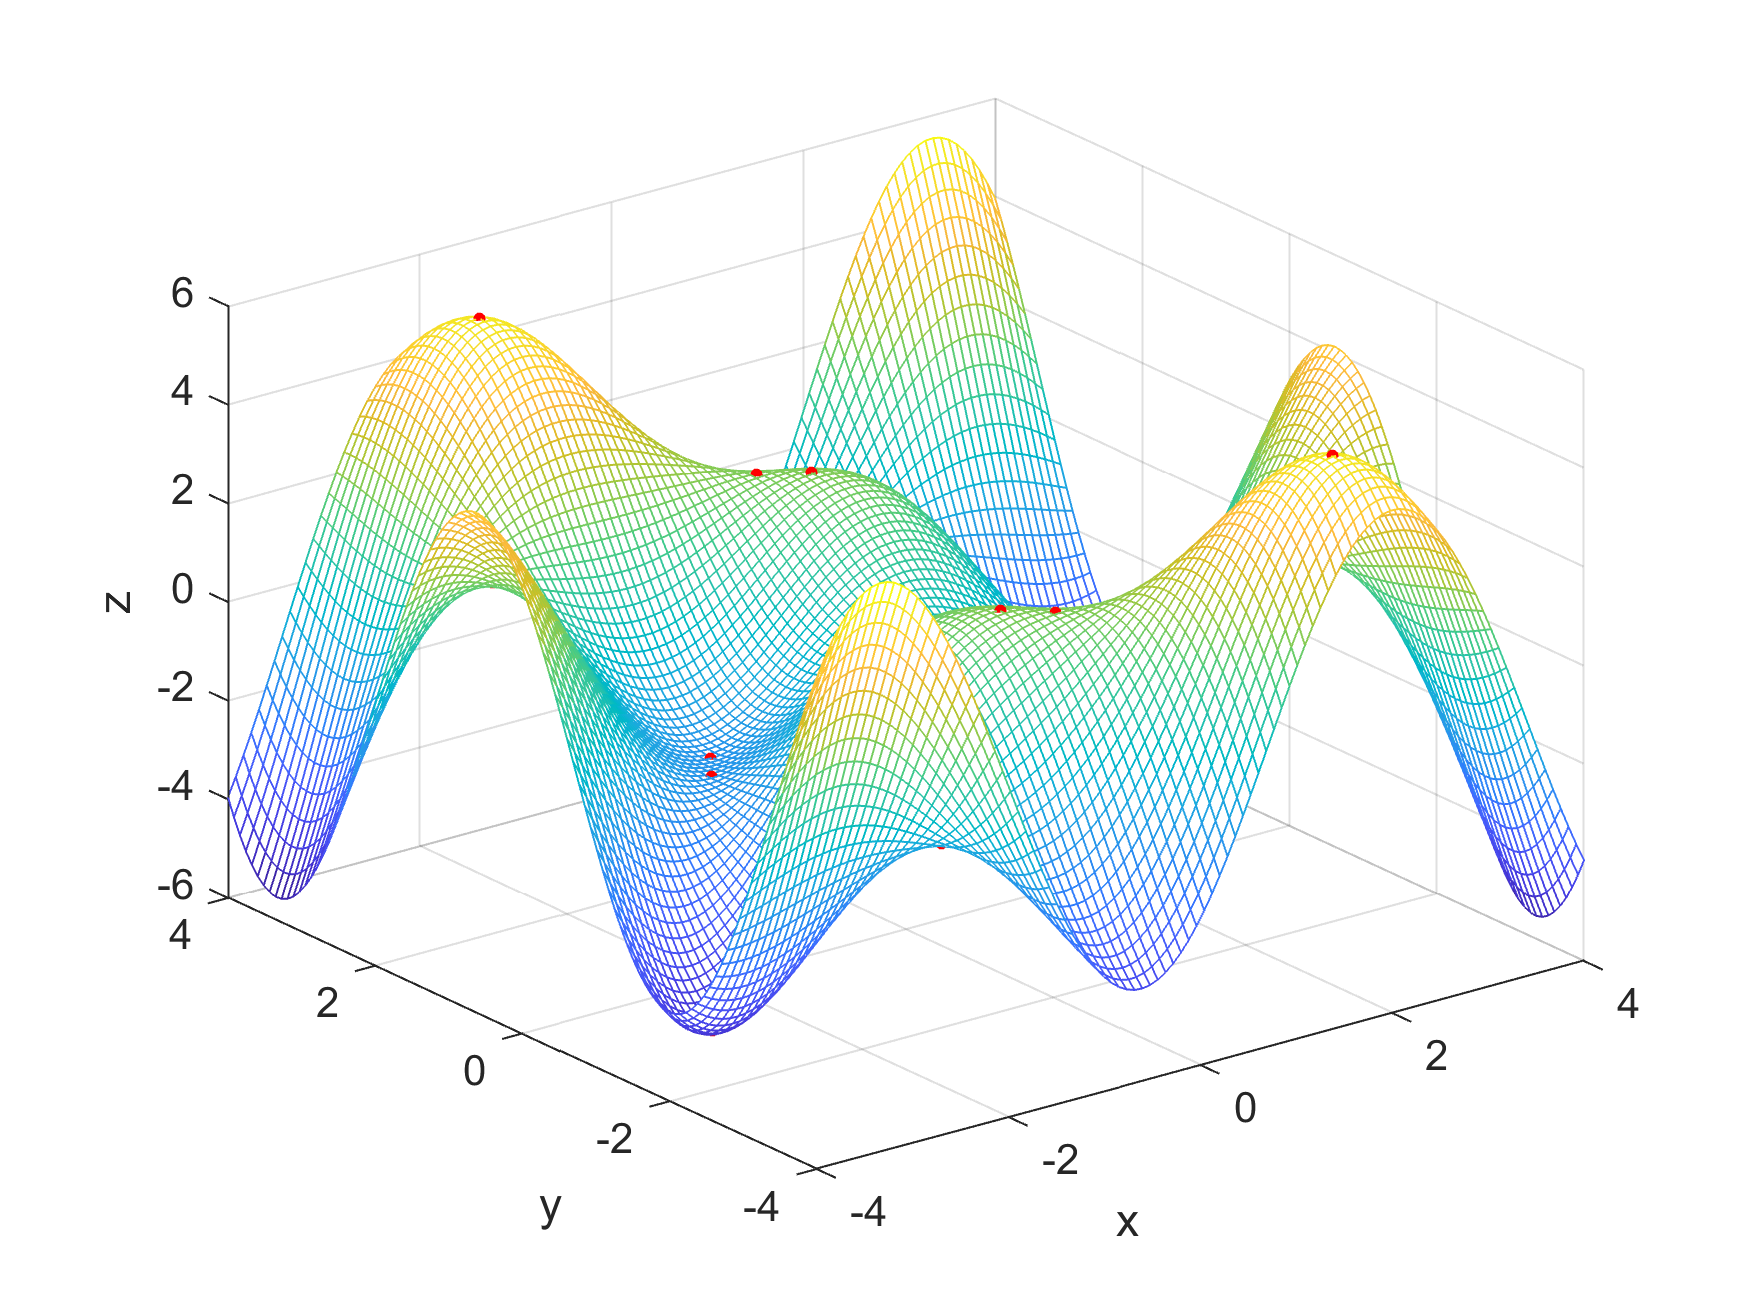
\includegraphics[width=12cm]{Q1/figures/3DplotWithPoints.png}
\end{figure}
\begin{figure}[H]
	\caption{Contour figure of function}
	\centering
	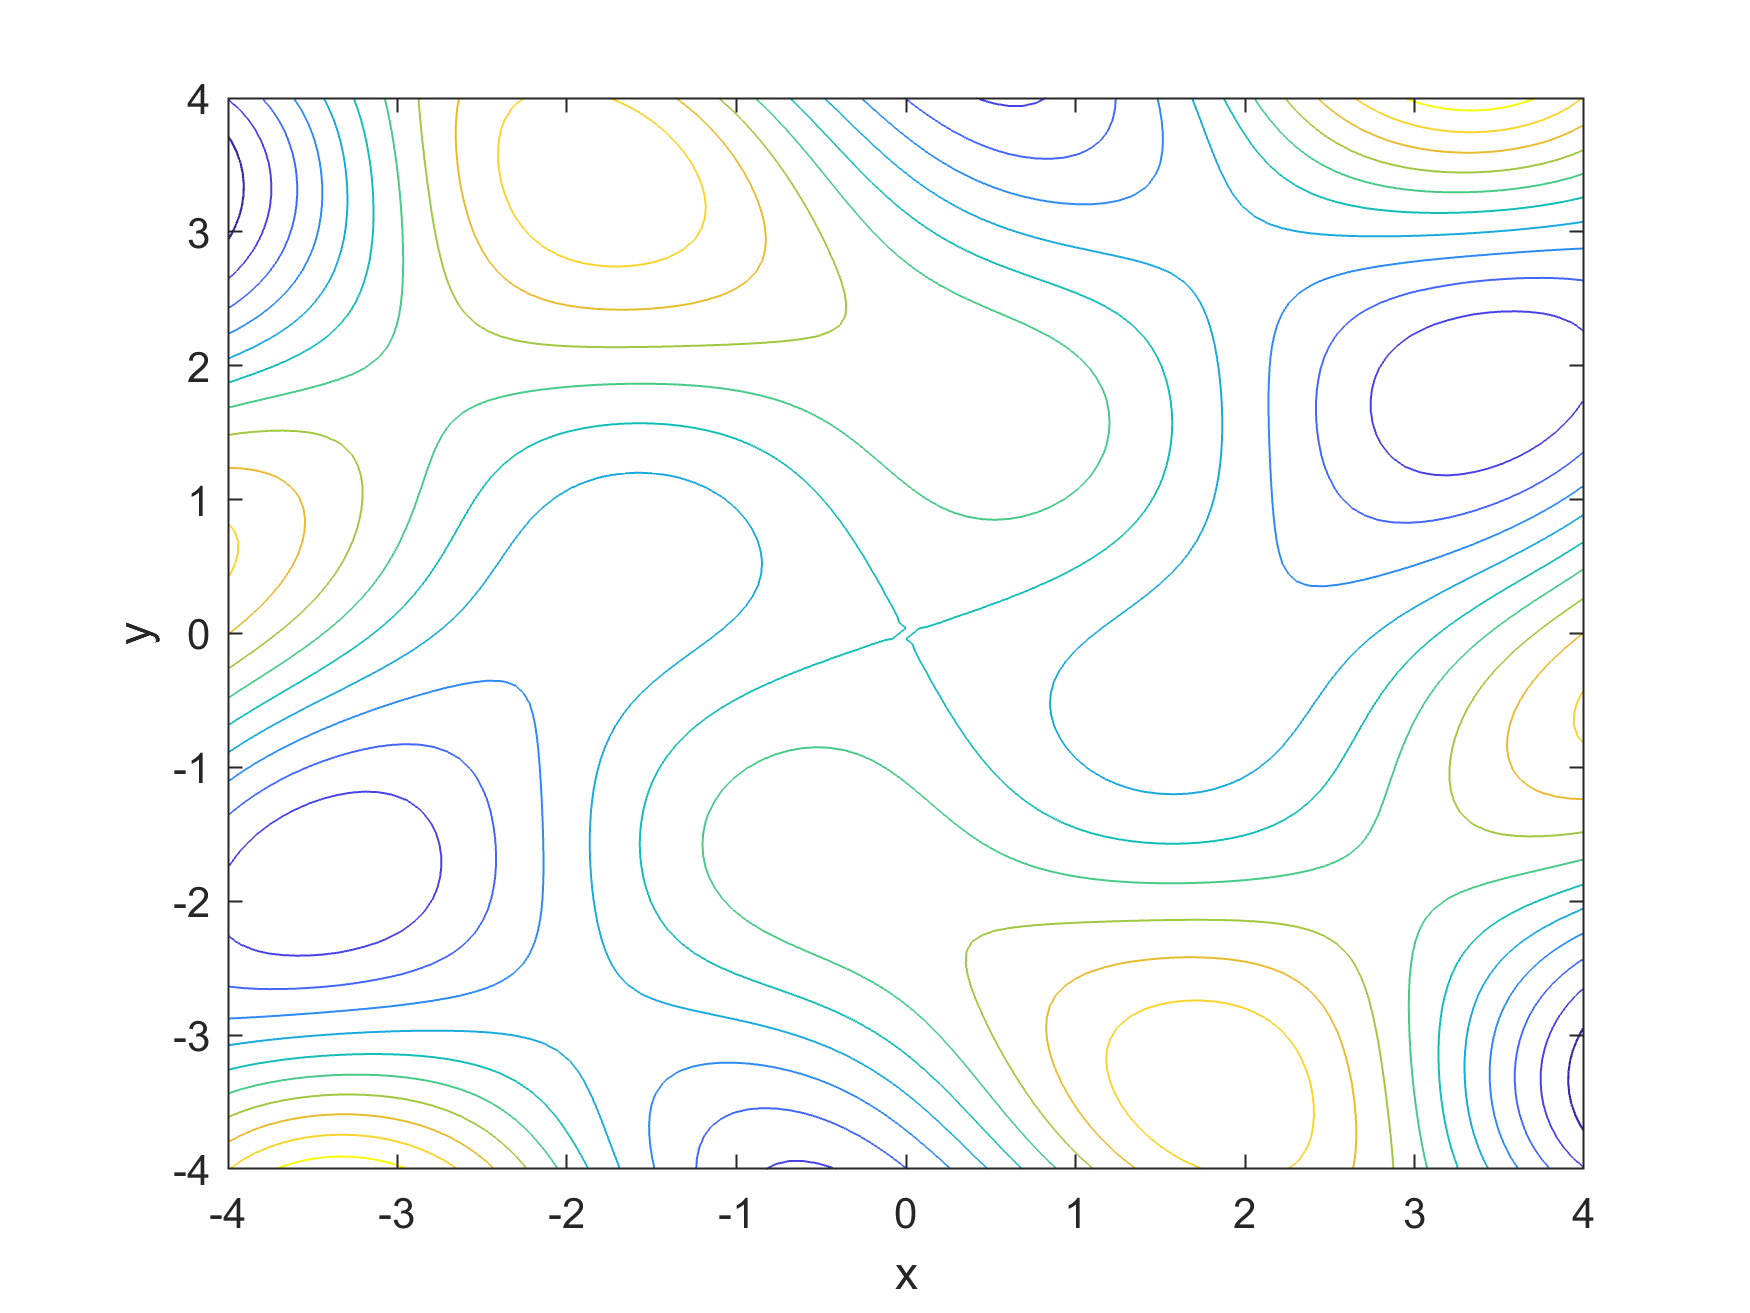
\includegraphics[width=12cm]{Q1/figures/Contour.png}
\end{figure}
\begin{figure}[H]
	\caption{Contour figure of function with Points}
	\centering
	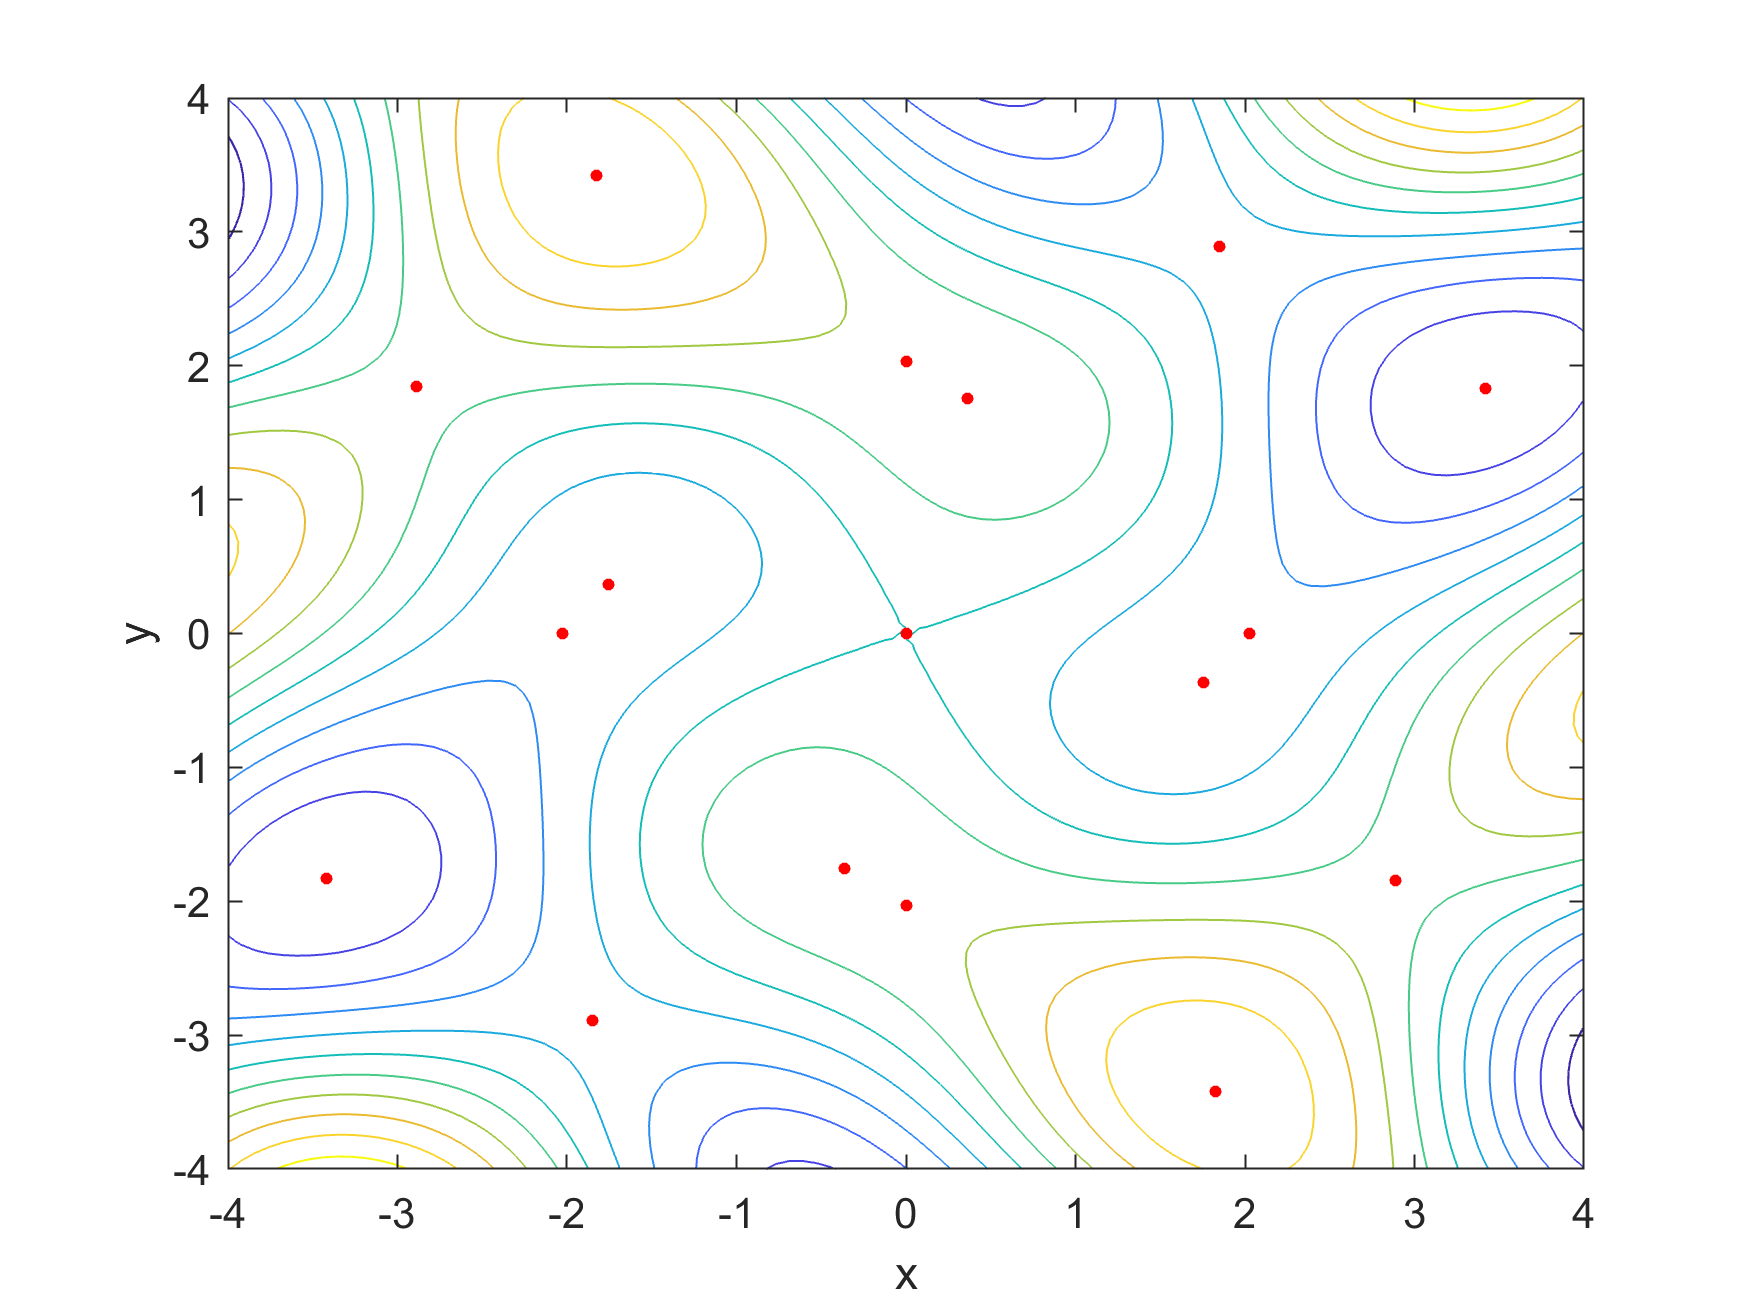
\includegraphics[width=12cm]{Q1/figures/ContourWithPoints.png}
\end{figure}


	\newpage
	\item 
	$z = f(x, y) = x^3 - 3xy^2$ \\
Gradient of f(x, y):
$$\vec{\nabla} f = \begin{bmatrix}
	\dfrac{\partial f}{\partial x} \\[6pt]
	\dfrac{\partial f}{\partial y}
\end{bmatrix} $$
$$\vec{\nabla} f = \begin{bmatrix}
	3x^2 - 3y^2 \\
	-6xy
\end{bmatrix} $$
Two linear equations with two unknowns.
$$	3x^2 - 3y^2 =  0 $$
$$-6xy = 0$$
Answers is $x = 0$ and $y = 0$.


Hessian matrix:
$$H = \dfrac{\partial^2 f}{\partial \vec{X}^2} = \begin{bmatrix}
	\dfrac{\partial^2 f}{\partial x^2} & \dfrac{\partial^2 f}{\partial xy} \\[6pt]
	\dfrac{\partial^2 f}{\partial yx}  & \dfrac{\partial f}{\partial y^2}
\end{bmatrix} $$
$$H = \begin{bmatrix}
	6x & -6y \\
   -6y & -6x
\end{bmatrix}$$



In $x = 0$ and $y = 0$ Hessian matrix in :
$$H = \begin{bmatrix}
	0 & 0 \\
	0 & 0
\end{bmatrix}$$
so this point is saddle point.
\begin{figure}[H]
	\caption{3D figure of function}
	\centering
	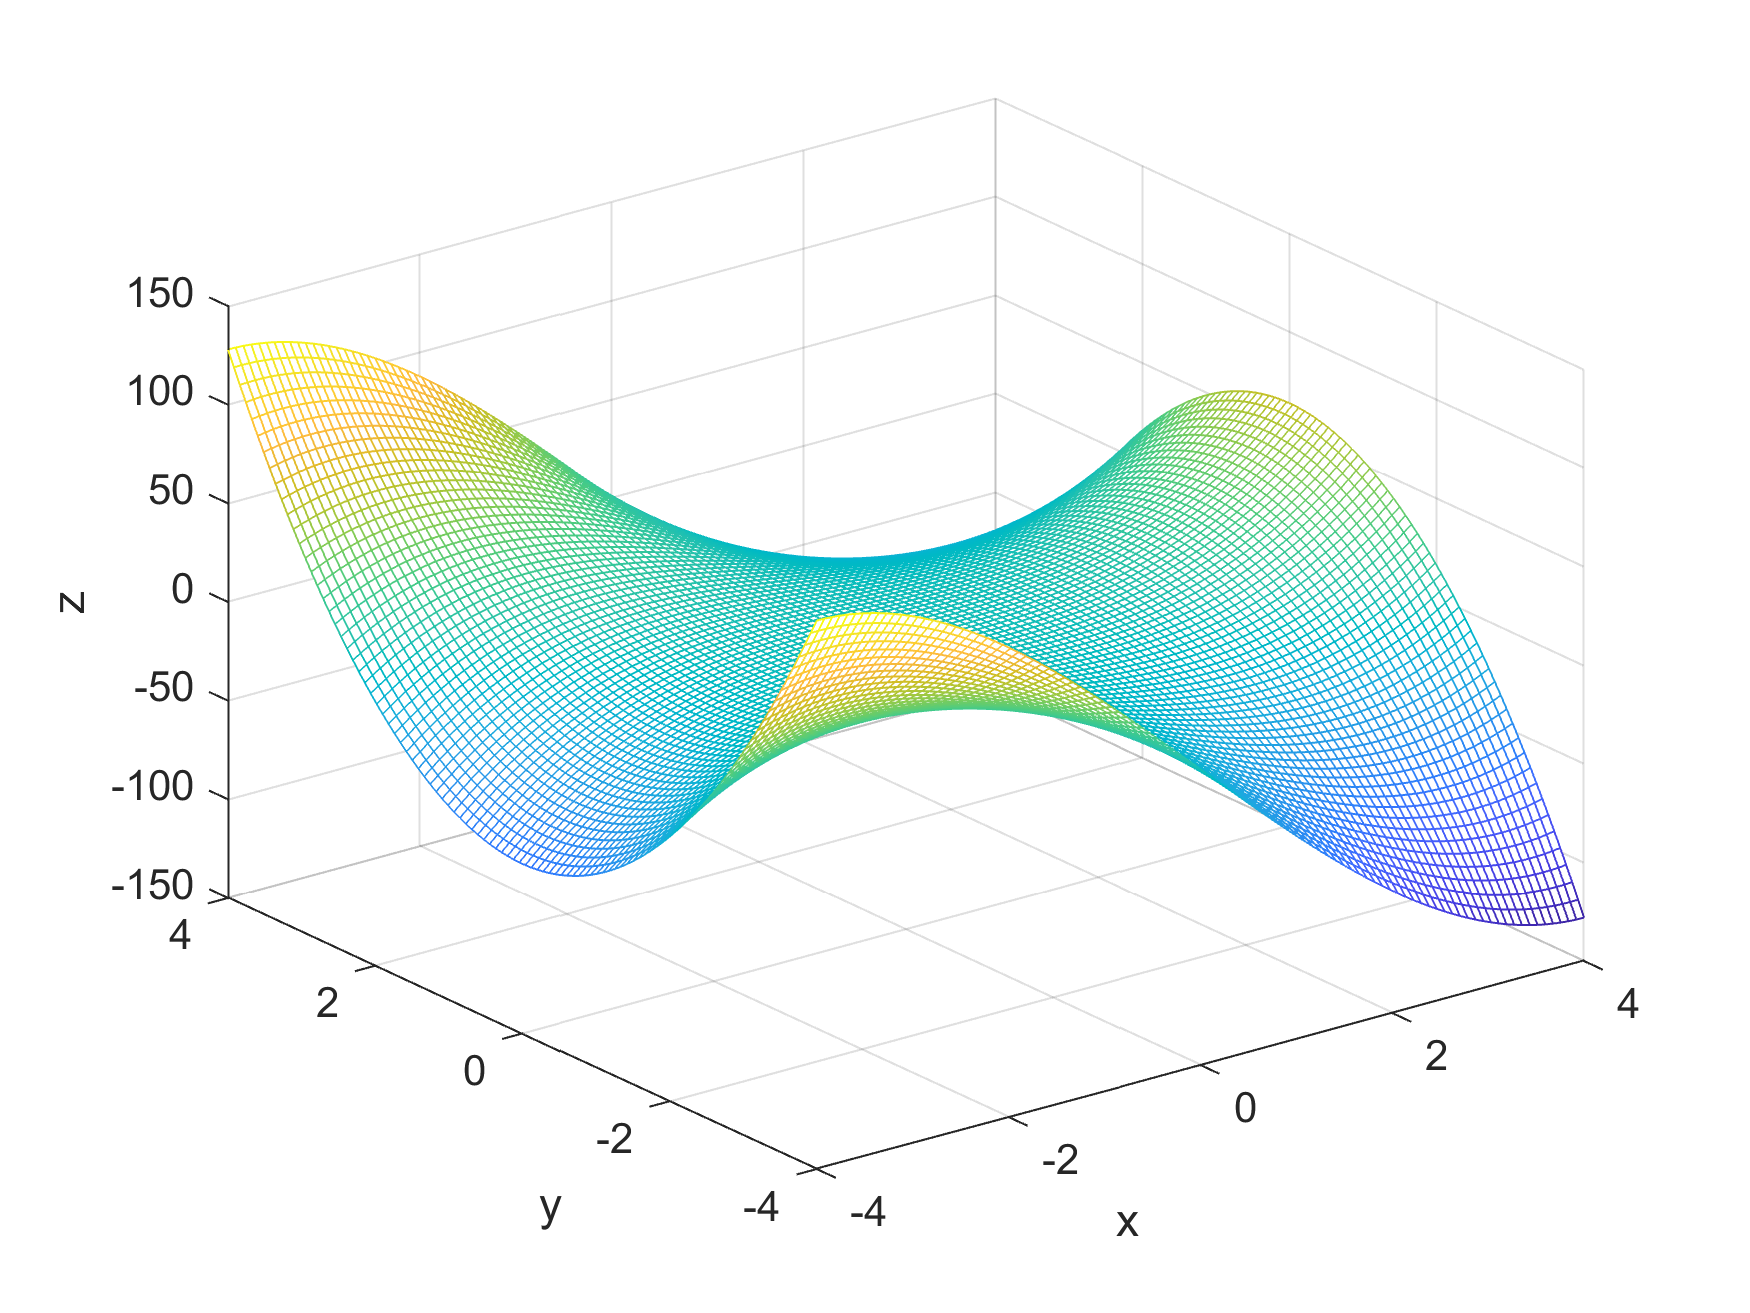
\includegraphics[width=12cm]{Q1/figures/3DplotQ1b.png}
\end{figure}

\begin{figure}[H]
	\caption{3D figure of function with Points}
	\centering
	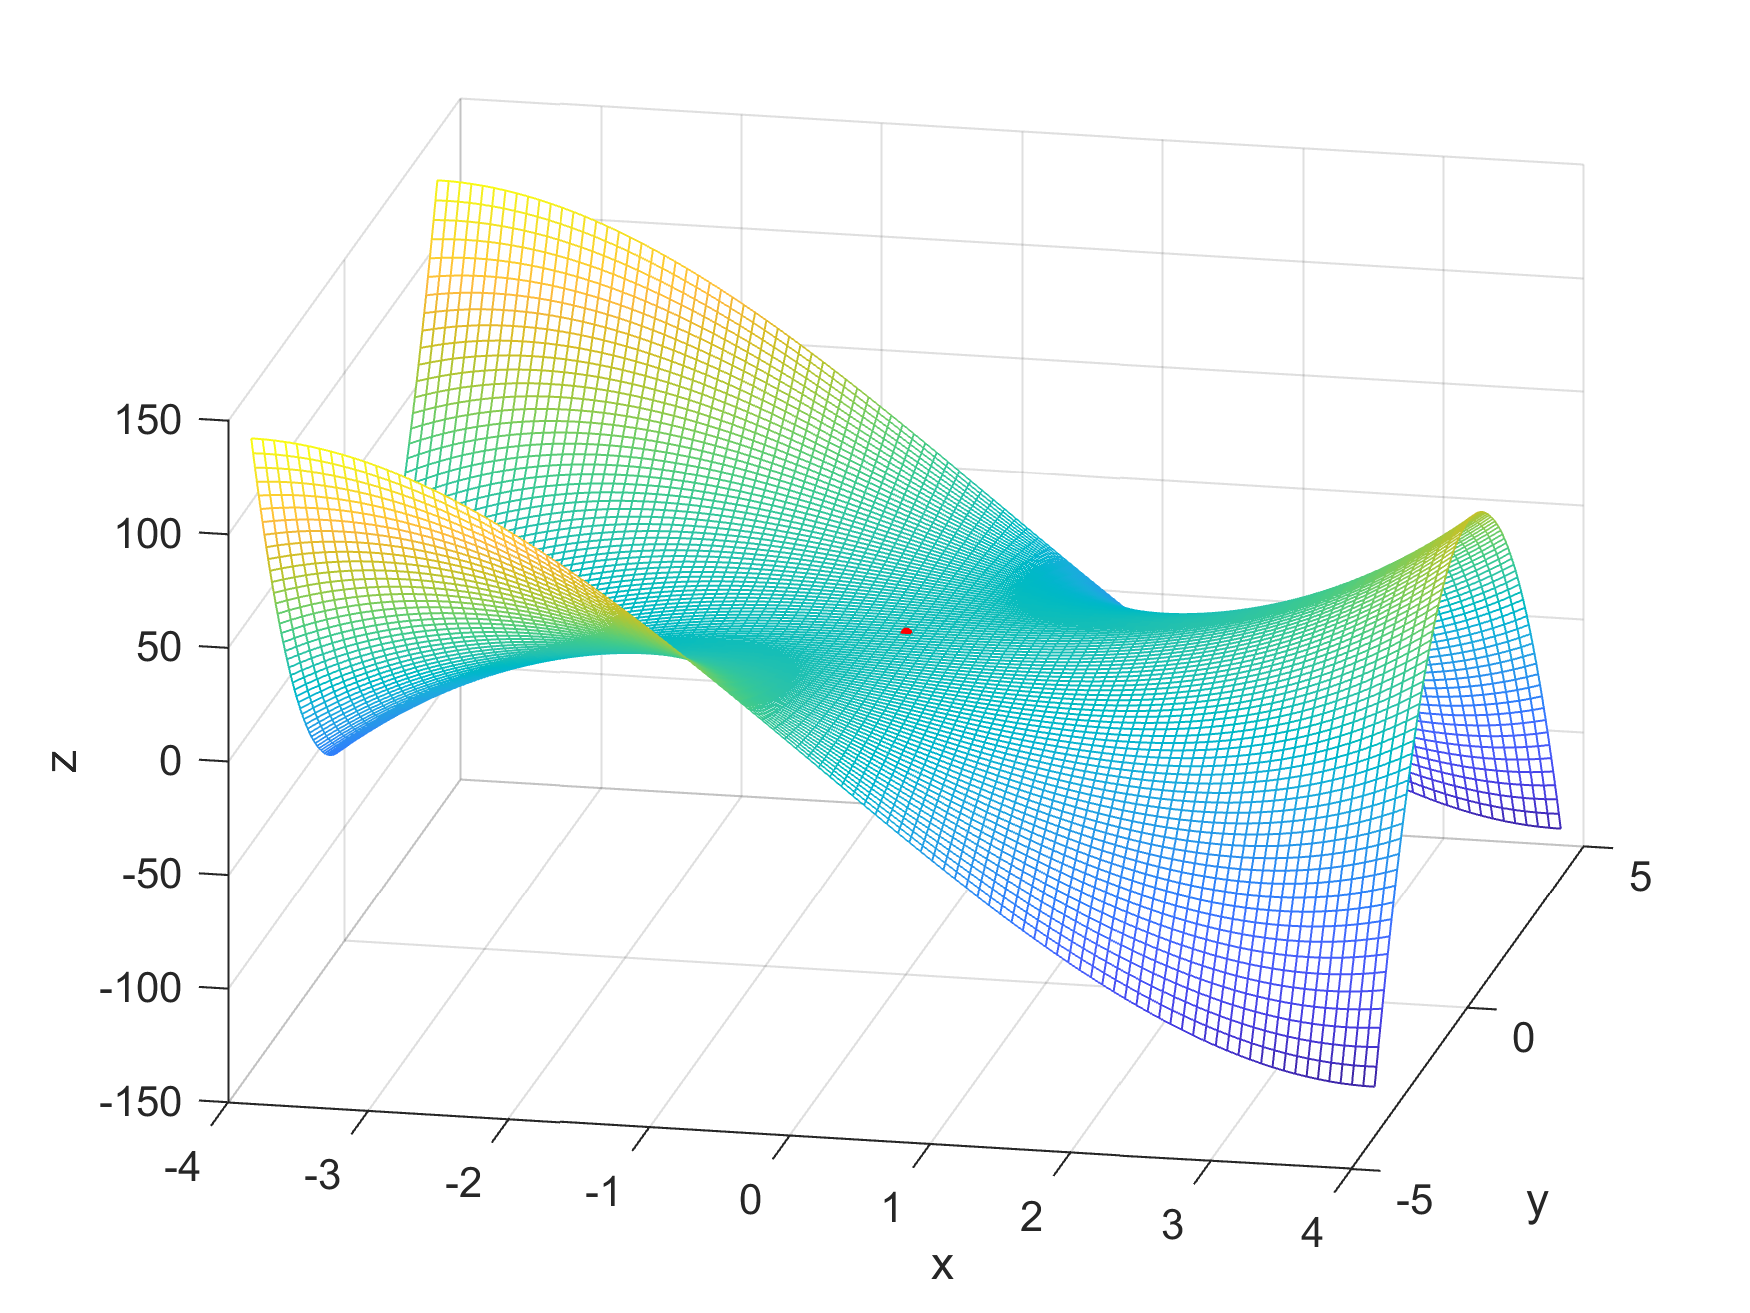
\includegraphics[width=12cm]{Q1/figures/3DplotWithPointsTashihQ1b.png}
\end{figure}

\begin{figure}[H]
	\caption{Contour figure of function}
	\centering
	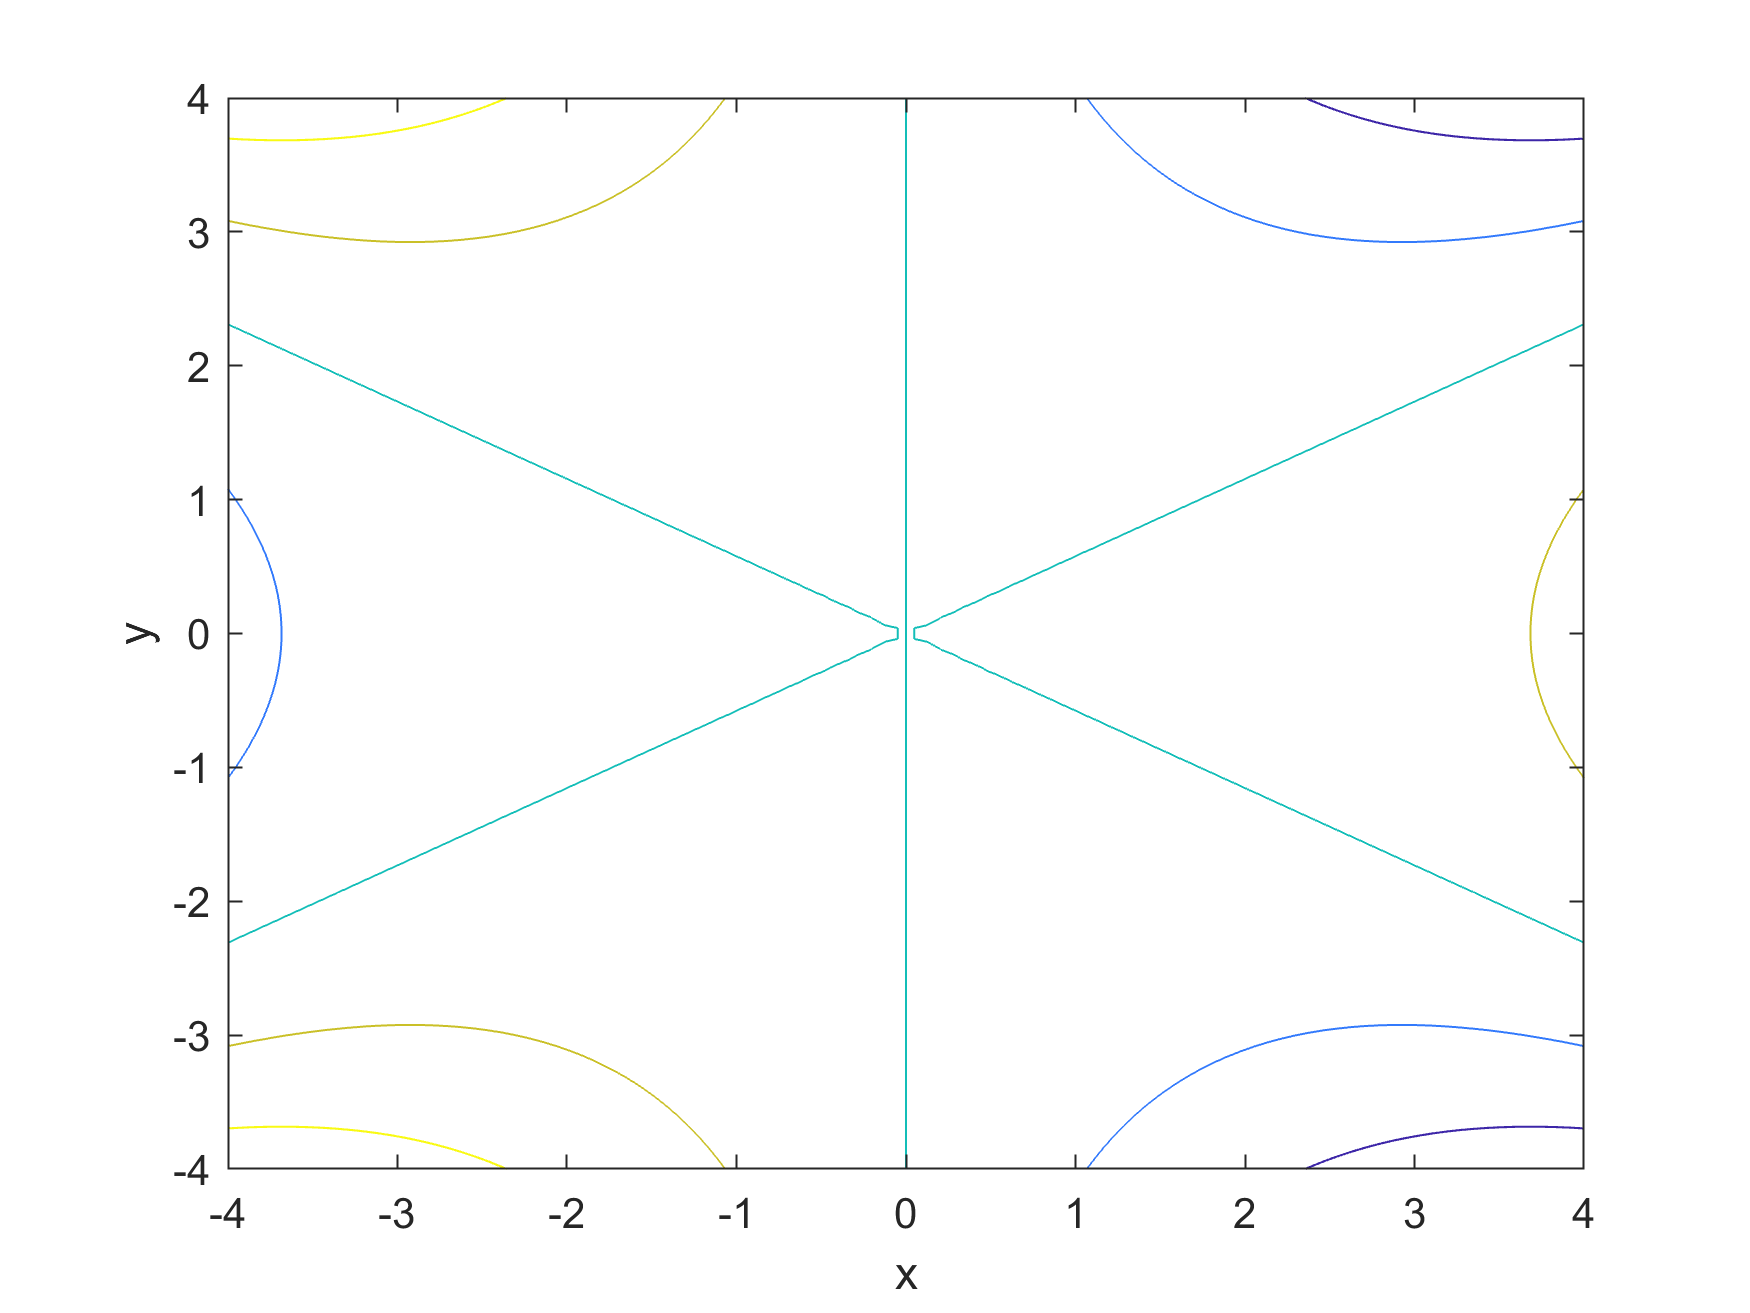
\includegraphics[width=12cm]{Q1/figures/ContourQ1b.png}
\end{figure}
\begin{figure}[H]
	\caption{Contour figure of function with Points}
	\centering
	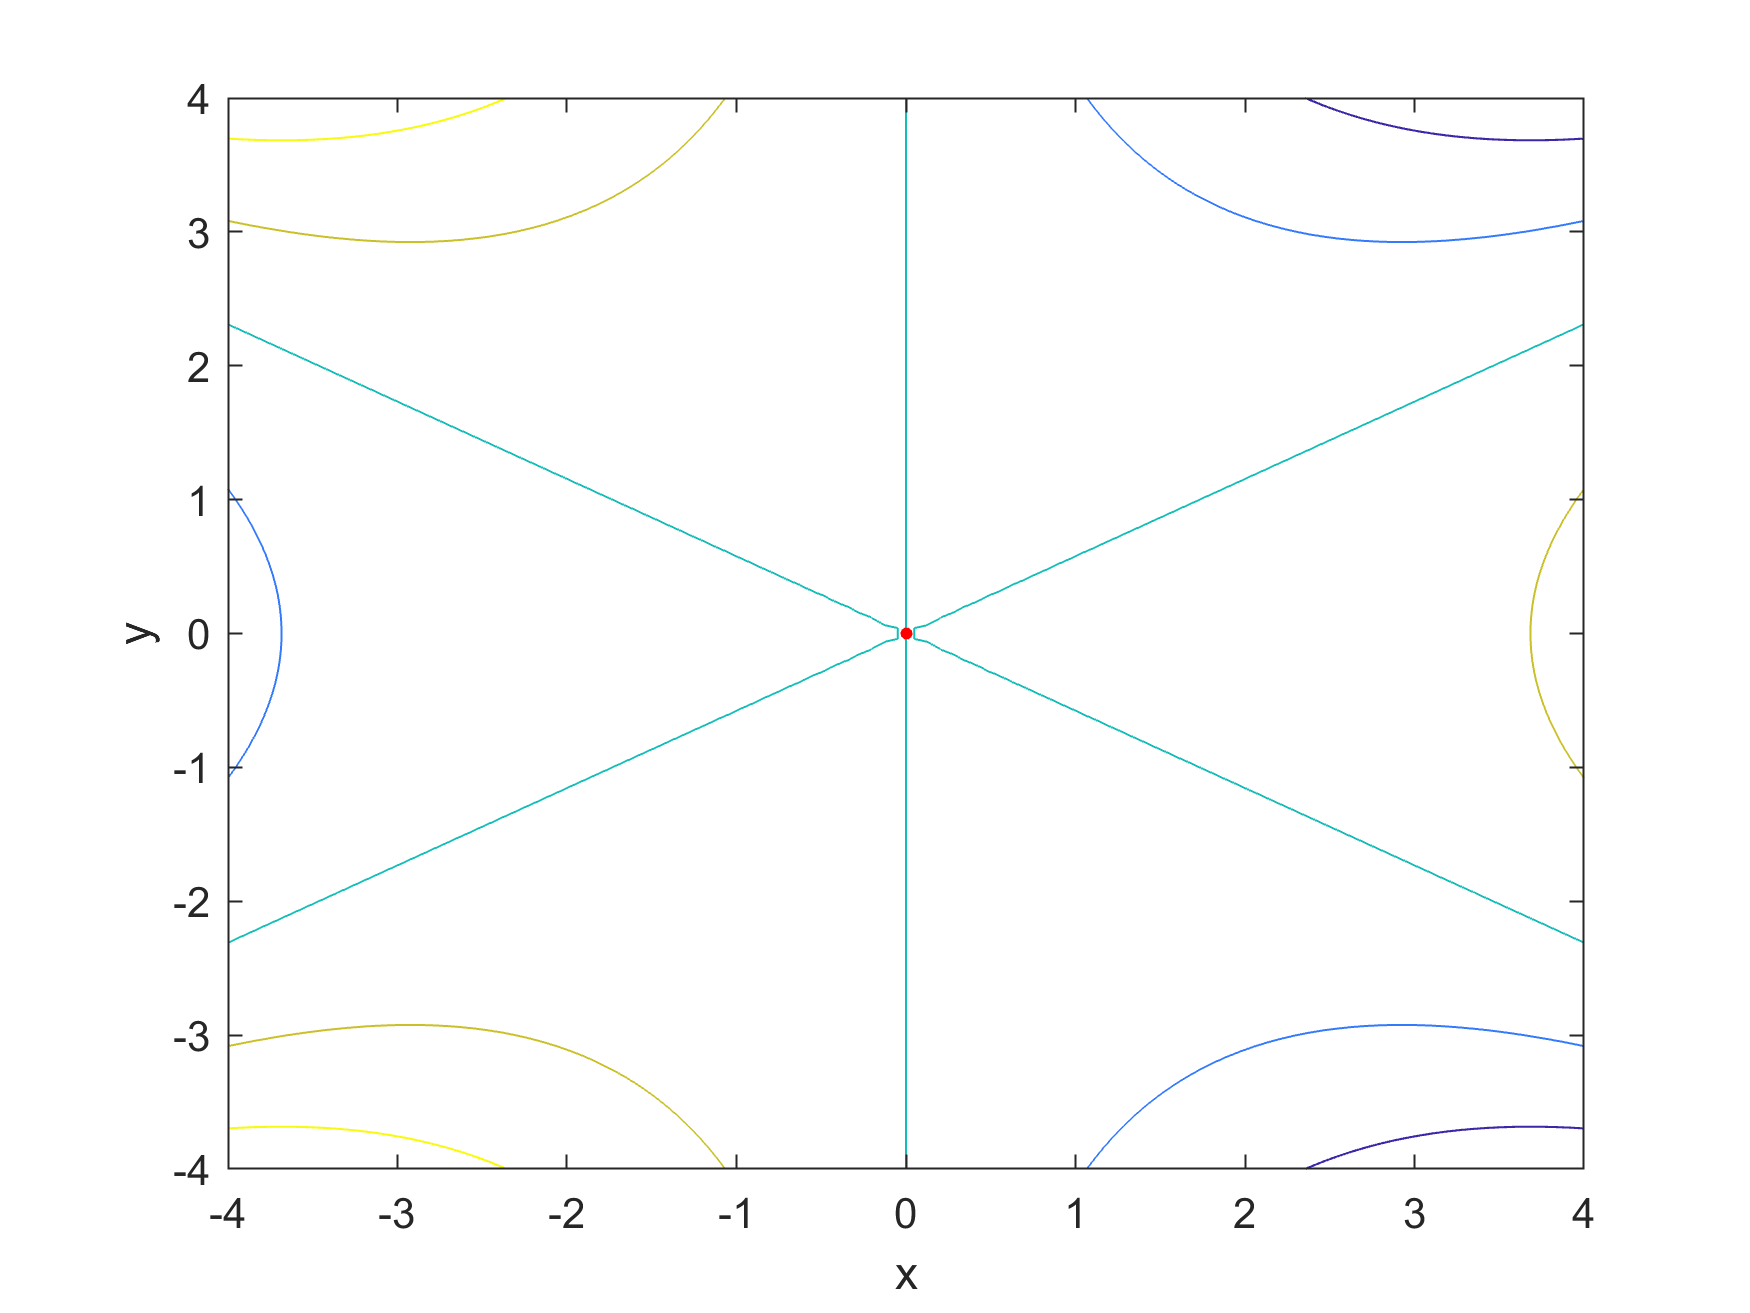
\includegraphics[width=12cm]{Q1/figures/ContourWithPointsQ1b.png}
\end{figure}

	\newpage
	\item 
	$z = f(x_1, x_2, x_3) = x_1^2 + x_1x_2 - 4x_2^2-x_3^2 + 3x_2x_3$ \\
Gradient of $f(x_1, x_2, x_3)$:
$$\vec{\nabla} f = \dfrac{\partial f}{\partial \vec{X}}= \begin{bmatrix}
	\dfrac{\partial f}{\partial x_1} \\[8pt]
	\dfrac{\partial f}{\partial x_2} \\[8pt]
	\dfrac{\partial f}{\partial x_3} \\
\end{bmatrix} $$
$$\vec{\nabla} f =   \begin{bmatrix}
	2x_1 + x_2 \\
	x_1 -8x_2 + 3x_3 \\
	3x_2 - 2x_3
\end{bmatrix}  = \vec{0}$$
Three linear equations with Three unknowns.
$$	2x_1 + x_2 = 0 $$
$$x_1 -8x_2 + 3x_3 = 0$$
$$3x_2 - 2x_3 = 0 $$
Answers is $x_1 = x_2 = x_3 = 0$
Hessian matrix:
$$H = \dfrac{\partial^2 f}{\partial \vec{X}^2} = \begin{bmatrix}
	\dfrac{\partial^2 f}{\partial x_1^2} & \dfrac{\partial^2 f}{\partial x_1x_2} & \dfrac{\partial^2 f}{\partial x_1x_3} \\[8pt]
	\dfrac{\partial^2 f}{\partial x_2x_1}  & \dfrac{\partial f}{\partial x_2^2} & \dfrac{\partial^2 f}{\partial x_2x_3}  \\[8pt]
		\dfrac{\partial^2 f}{\partial x_3x_1}  & \dfrac{\partial f}{\partial x_3x_2} & \dfrac{\partial^2 f}{\partial x_3^2} 
\end{bmatrix} $$
$$H = \begin{bmatrix}
	2 & 1 & 0 \\
	1 & -8 & 3 \\
	0 & 3 & -2
\end{bmatrix}$$
All Hessian eigenvalues are:
$$eig(H) = \begin{bmatrix}
	-9.3182  \\
	-0.8077 \\
	2.1259
\end{bmatrix}$$
So $(0, 0, 0)$ is a saddle point.
\end{enumerate}
\newpage
\section*{Problem 2}
$$\min f(x, y, z) = x^2 + y^2 + z^ 2$$
subject to : $$z = \sin(x) + \cos(y)$$
\begin{enumerate}[label=(\alph*)]
	\item 
	Direct Substitution:


$z = \sin(x) + \cos(y) \xrightarrow{f(x, y, z) = x^2 + y^2 + z^ 2}
f(\vec{X}) = f(x, y) = x^2 + y^2 + (\sin(x)+\cos(y))^2
$


$f(x, y) = x^2 + y^2 + \sin(x)^2 + 2\sin(x)\cos(y) + \cos(y)^2$
Gradient of f(x, y):
$$\vec{\nabla} f = \begin{bmatrix}
	\dfrac{\partial f}{\partial x} \\[6pt]
	\dfrac{\partial f}{\partial y}
\end{bmatrix} $$
$$\vec{\nabla} f = \begin{bmatrix}
	2x + 2\cos(x)\cos(y) + 2\cos(x)\sin(x) \\
	2y - 2\cos(y)\sin(y) - 2\sin(x)\sin(y)
\end{bmatrix} $$
$$	2x + 2\cos(x)\cos(y) + 2\cos(x)\sin(x)=  0 $$
$$2y - 2\cos(y)\sin(y) - 2\sin(x)\sin(y) 0$$
Above equation solved in MATLAB and code (Q2\_a.m) has attached to homework.


$x = -0.47872, \quad y = 0.0 \to z =  $



	\item 
	Lagrange multipliers


$\min \mathcal{L}(\vec{X}, \vec{\lambda}) = f(\vec{X}) +\vec{\lambda}^T \vec{g}$

necessary condition:
$$\vec{\nabla} \mathcal{L}  =  \begin{bmatrix}
	 \vec{\nabla}_{\vec{X}} \mathcal{L} \\[6pt]
	 \vec{\nabla}_{\vec{\lambda}} \mathcal{L}
\end{bmatrix} = \begin{bmatrix}
\dfrac{\partial \mathcal{L}}{\partial \vec{X}} \\[10pt]
\dfrac{\partial \mathcal{L}}{\partial \vec{\lambda}}
\end{bmatrix} = \vec{0}$$
$f(\vec{X}) = x^2 + y^2 + z^2, \quad  g(\vec{X}) = \sin(x) + \cos(y) - z = 0$
$$\min \mathcal{L}(\vec{X}, \vec{\lambda}) = x^2 + y^2 + z^2 + \lambda (\sin(x) + \cos(y) - z)$$
$$\vec{\nabla} \mathcal{L} = \begin{bmatrix}
	\dfrac{\partial \mathcal{L}}{\partial x} \\[10pt]
	\dfrac{\partial \mathcal{L}}{\partial y} \\[10pt]
	\dfrac{\partial \mathcal{L}}{\partial z} \\[10pt]
	\dfrac{\partial \mathcal{L}}{\partial \lambda}
\end{bmatrix}  = \begin{bmatrix}
2x + \lambda\cos(x) \\
2y - \lambda\sin(y) \\
2z - \lambda \\
\sin(x) + \cos(y) -z
\end{bmatrix}$$
Above equation solved in MATLAB and code (Q2\_b.m) has attached to homework.
\begin{table}[H]
	\caption {Answers} \label{ans} 
	\begin{center}
		\begin{tabular}{| l | l | l |}
			\hline
			  x & y & z \TBstrut \\
			  \hline
			-0.47872 & 0.000 & 0.5393 \Tstrut\\
			\hline
		\end{tabular}
	\end{center}
\end{table}
\end{enumerate}


\newpage
\section*{Problem 3}
$$\min f(x_1, x_2, y_1, y_2) = (x_1- x_2)^2 + (y_1 - y_2)^2$$
subject to : $$y = x^2, \quad y = x-1$$
\begin{enumerate}[label=(\alph*)]
	\item 
	Direct Substitution:



$f(x_1, x_2, y_1, y_2) = (x_1- x_2)^2 + (y_1 - y_2)^2 \xrightarrow{y_1 = x_1^2, \quad y_2 = x_2-1} f(x_1, x_2) = (x_1- x_2)^2 + (x_1^2 - (x_2-1)^2)^2$
$$f(x_1, x_2) = x_1^4 - 2x_1^2x_2^2 + 4x_1^2x_2 - x_1^2 - 2x_1x_2 + x_2^4 - 4x_2^3 + 7x_2^2 - 4x_2 + 1$$


Gradient of $f(x_1, x_2)$:
$$\vec{\nabla} f = \begin{bmatrix}
	\dfrac{\partial f}{\partial x_1} \\[6pt]
	\dfrac{\partial f}{\partial x_2}
\end{bmatrix} $$
$$\vec{\nabla} f = \begin{bmatrix}
	4x_1^3 - 4x_1x_2^2 + 8x_1x_2 - 2x_1 - 2x_2 \\
	- 4x_1^2x_2 + 4x_1^2 - 2x_1 + 4x_2^3 - 12x_2^2 + 14x_2 - 4
\end{bmatrix} $$
Two nonlinear equations with two unknowns. We use MATLAB to solve this equations. MATLAB file (Q3\_a.m) is attached.
$$	4x_1^3 - 4x_1x_2^2 + 8x_1x_2 - 2x_1 - 2x_2 =  0 $$
$$- 4x_1^2x_2 + 4x_1^2 - 2x_1 + 4x_2^3 - 12x_2^2 + 14x_2 - 4 = 0$$
$x_1 = \dfrac{1}{2} \to y_1 = \dfrac{1}{4}, \quad x_2 = \dfrac{7}{8} \to y_2 = \dfrac{1}{8}$
\begin{table}[H]
	\caption {Answers} \label{ans} 
	\begin{center}
		\begin{tabular}{| l | l | l | l |}
			\hline
			$x_1$ & $y_1$ & $x_2$ & $y_2$ \TBstrut \\
			\hline
			$0.5$ & $0.25$ & $0.875$ & $0.125$ \Tstrut\\
			\hline
		\end{tabular}
	\end{center}
\end{table}


	\item 
	Lagrange multipliers:


$\min \mathcal{L}(\vec{X}, \vec{\lambda}) = f(\vec{X}) +\vec{\lambda}^T \vec{g}$
necessary condition:
$$\vec{\nabla} \mathcal{L}  =  \begin{bmatrix}
	 \vec{\nabla}_{\vec{X}} \mathcal{L} \\[6pt]
	 \vec{\nabla}_{\vec{\lambda}} \mathcal{L}
\end{bmatrix} = \begin{bmatrix}
\dfrac{\partial \mathcal{L}}{\partial \vec{X}} \\[10pt]
\dfrac{\partial \mathcal{L}}{\partial \vec{\lambda}}
\end{bmatrix} = \vec{0}$$
$f(\vec{X}) = (x_1- x_2)^2 + (y_1 - y_2)^2, \quad  g(\vec{X}) = \begin{bmatrix}
y_1-x_1^2 &
y_2-x_2+1
\end{bmatrix} = \vec{0}$
$$\min \mathcal{L}(\vec{X}, \vec{\lambda}) = (x_1- x_2)^2 + (y_1 - y_2)^2 + \lambda_1(y_1-x_1^2) + \lambda_2(y_2-x_2+1)$$
$$\vec{\nabla} \mathcal{L} = \begin{bmatrix}
	\dfrac{\partial \mathcal{L}}{\partial x_1} \\[10pt]
	\dfrac{\partial \mathcal{L}}{\partial y_1} \\[10pt]
	\dfrac{\partial \mathcal{L}}{\partial x_2} \\[10pt]
	\dfrac{\partial \mathcal{L}}{\partial y_2} \\[10pt]
	\dfrac{\partial \mathcal{L}}{\partial \lambda_1} \\[10pt]
	\dfrac{\partial \mathcal{L}}{\partial \lambda_2} 
\end{bmatrix}  =  \begin{bmatrix}
2x_1 - 2x_2 - 2\lambda_1x_1 \\
2y_1 - 2y_2 + \lambda_1 \\
2x_2 - 2x_1 - \lambda_2 \\
2y_2 - y_1 + \lambda_2 \\
y_1-x_1^2\\
y_2-x_2+1
\end{bmatrix} $$
Six nonlinear equations with six unknowns. We use MATLAB to solve this equations. MATLAB file (Q3\_b.m) is attached.
\begin{table}[H]
	\caption {Answers} \label{ans} 
	\begin{center}
		\begin{tabular}{| l | l | l | l | l | l | l |}
			\hline
			$x_1$ & $y_1$ & $x_2$ & $y_2$ &  $\lambda_1$&  $\lambda_2$ \TBstrut \\
			\hline
			$0.5$ & $0.25$ & $0.875$ & $-0.125$ & -0.75& 0.75 \Tstrut\\
			\hline
		\end{tabular}
	\end{center}
\end{table}

	\item 
	Calculus of Variation:


Euler–Lagrange equation:
$$g_x - \dfrac{d}{dt}g_{\dot{x}} = 0$$
In problem g function is that we must minimize is:
$$g(\dot{x}, x, t) = g(\dot{x}) = \sqrt{1+\dot{x}^2} = $$
$$\to \dfrac{\partial g_{\dot{x}}}{\partial \dot{x}} \dfrac{\dot{x}}{dt} = 0 \to g_{\dot{x}\dot{x}}\ddot{x} = 0 $$
The solution is line:
$$\to x(t) = c_1t+ c_2$$
Boundary condition:



Initial time: 
$\theta(t) = t^2 $
$$(g + (\dot{\theta}-\dot{x})g_{\dot{x}}) \vert_{t = t_0}= 0 \to \sqrt{1+\dot{x}^2} + (2t -\dot{x} )\dfrac{\dot{x}}{\sqrt{1+\dot{x}^2}}\vert_{t = t_0} = 0 \to t_0 = -\dfrac{1}{2\dot{x}}\vert_{t = t_0}$$
Final time: 
$\theta(t) = t-1 $
$$(g + (\dot{\theta}-\dot{x})g_{\dot{x}})\vert_{t = t_f}  = 0 \to \sqrt{1+\dot{x}^2} + (1-\dot{x}) \dfrac{\dot{x}}{\sqrt{1+\dot{x}^2}}\vert_{t = t_f} = 0 \to \dot{x}_f = -1$$
Because of x function $\dot{x}$ is constant in $t_0 \to t_f$,
$$\to c_1 = -1\\
\to t_0 = \dfrac{1}{2\dot{x}}\vert_{t = t_0} =-\dfrac{1}{2c_1} = \dfrac12 \to x_0 = \frac14 $$ 
$$x(t) = c_1t+c_2 \to x(t_0) = c_1t_0 + c_2 \to c_2 = 0.75$$
Final time:
$$x(t_f) = \theta(t_f) \to -t_f + 0.75 = t_f-1 \to t_f = 0.875 \to \xrightarrow{x(t) = -t+0.75} x_f = -0.125$$
Answer:
$$x(t) = -t+0.75 t_0 \to t_f$$

\begin{table}[H]
	\caption {Answers} \label{ans} 
	\begin{center}
		\begin{tabular}{| l | l | l | l |}
			\hline
			$t_0$ & $x_0$ & $t_f$ & $x_f$ \TBstrut \\
			\hline
			$0.5$ & $0.25$ & $0.875$ & $-0.125$ \Tstrut\\
			\hline
		\end{tabular}
	\end{center}
\end{table}
\begin{figure}[H]
	\caption{Answer function}
	\centering
	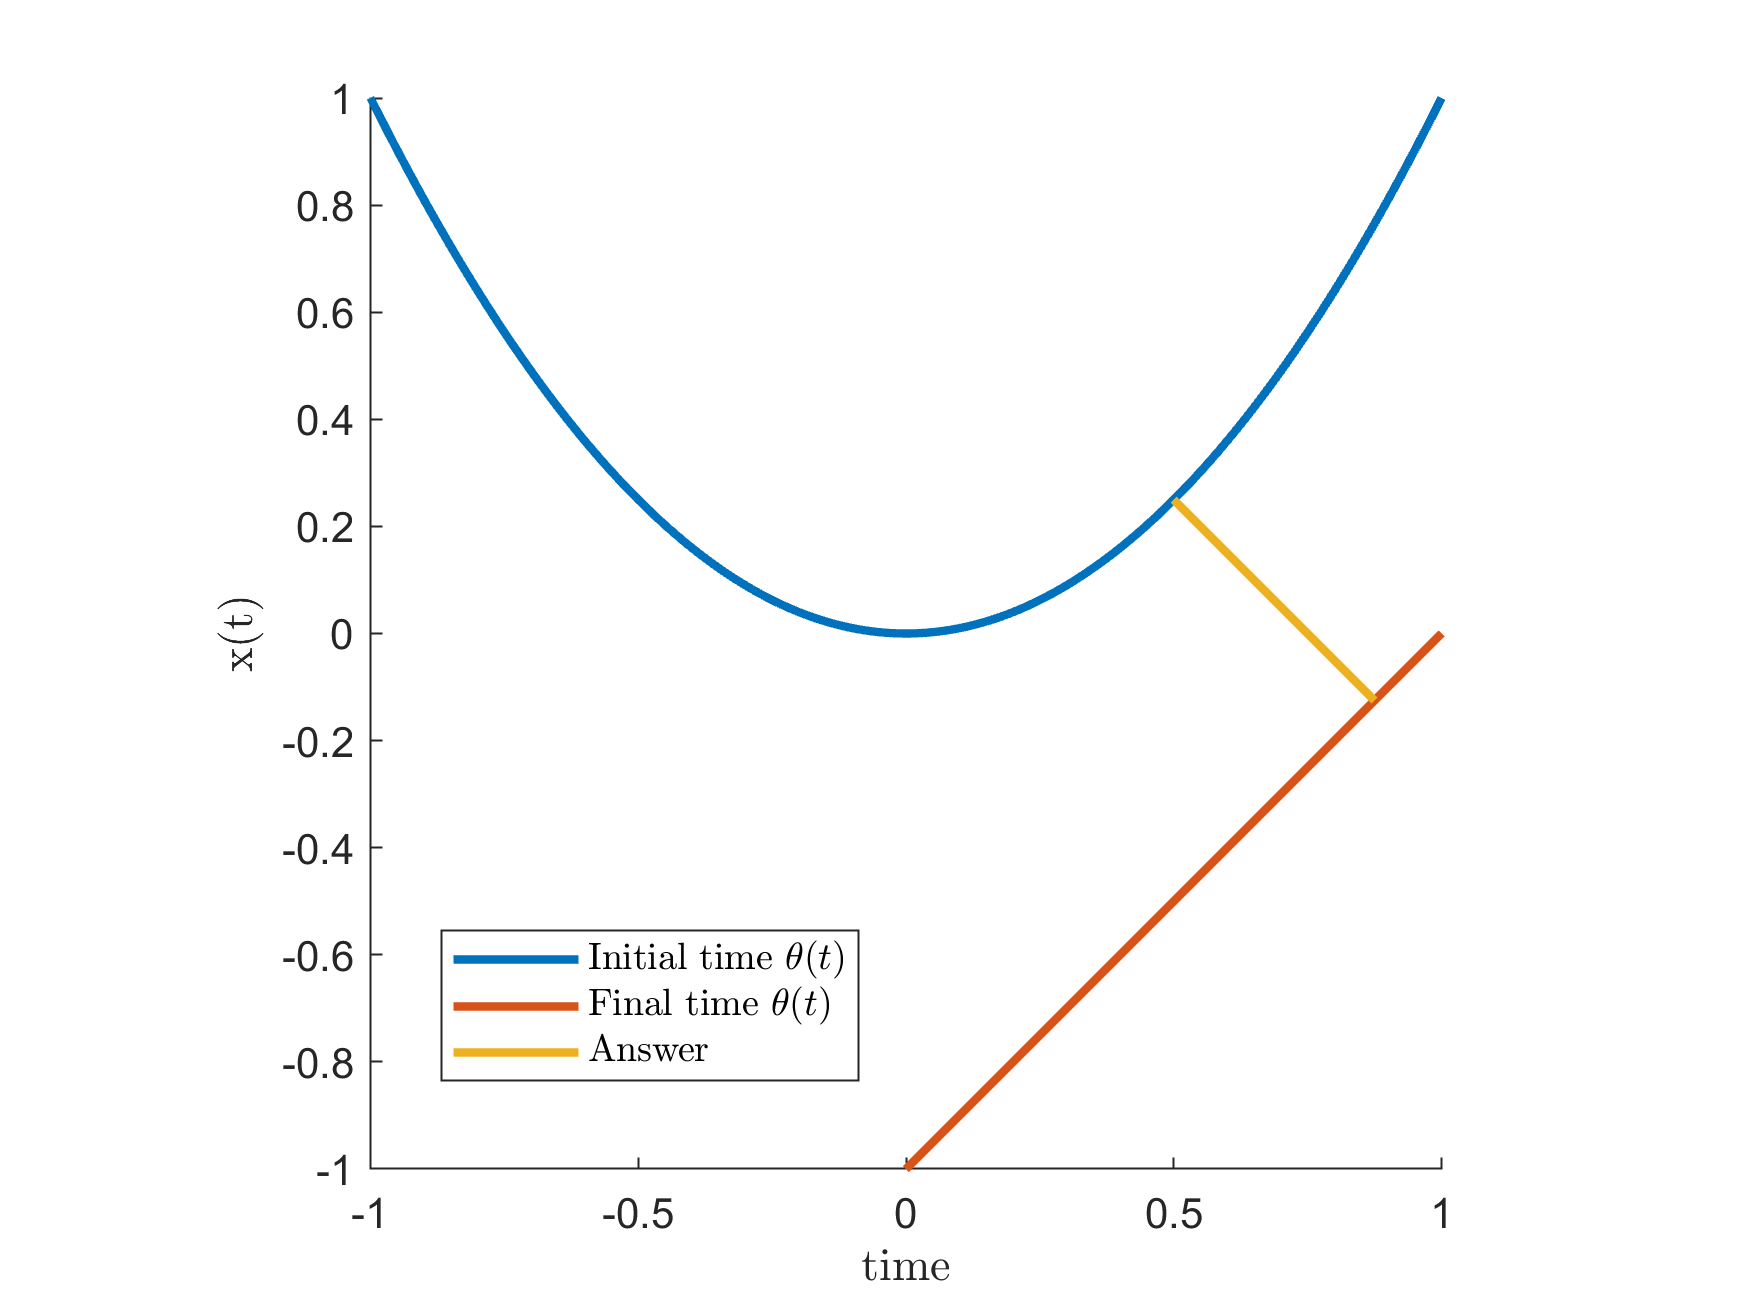
\includegraphics[width=12cm]{Q3/figures/Q3figureFix.png}
\end{figure}

	\item 
	hi
\end{enumerate}
\end{document}
